\documentclass[a4paper,10pt,twoside]{article}
%\usepackage{amssymb}
%\usepackage{amsthm}
\usepackage[polish]{babel}
\usepackage[utf8]{inputenc}
\usepackage[T1]{fontenc}
\usepackage{indentfirst}
\usepackage[top=2.5cm, bottom=2.5cm, left=2.5cm, right=2.5cm]{geometry}
\usepackage{booktabs}
\usepackage{graphicx}
\usepackage{float}
\usepackage{wrapfig}
%\usepackage{xcolor}
\usepackage{amsmath}

\begin{document}

\newgeometry{top=1.5cm,bottom=2.5cm,left=2.5cm,right=2.5cm}
\begin{center}
\bgroup
\def\arraystretch{1.5}
\begin{tabular}{|c|c|c|c|c|c|}
	\hline
	EAIiIB & \multicolumn{2}{|c|}{\begin{tabular}{@{}c@{}}Marcin Nalepa \\ Przemysław Trybała\end{tabular}} & Rok II & Grupa 5 & Zespół 3 \\
	\hline
	\multicolumn{3}{|c|}{\begin{tabular}{c}Temat: \\ Moduł Younga \end{tabular}} & 
	\multicolumn{3}{|c|}{\begin{tabular}{c}Numer ćwiczenia: \\ 11 \end{tabular}} \\
	\hline
	\begin{tabular}{@{}c@{}}Data wykonania\\25.11.2015 r.\end{tabular} & \begin{tabular}{@{}c@{}}Data oddania\\9.12.2015 r.\end{tabular} & 
	\begin{tabular}{c}Zwrot do\\poprawki\\\phantom{data} \end{tabular} & \begin{tabular}{c}Data oddania\\\phantom{data}\end{tabular} &
	\begin{tabular}{c}Data zaliczenia\\\phantom{data}\end{tabular} & \begin{tabular}{c}Ocena\\\phantom{ocena}\end{tabular} \\[4ex]
	\hline
\end{tabular}
\egroup
\end{center}

\section{Cel ćwiczenia}
Celem ćwiczenia jest wyznaczenie modułu Younga metodą statyczną czyli za pomocą
mierzenia wydłużenia drutu, wykonanego z danego materiału i obciążonego stałą siłą.

\section{Wstęp teoretyczny}
Wszystkie ciała, w mniejszym lub większym stopniu, ulegają odkształceniom pod wpływem działających na nie sił.
Jeśli odkształcenia te znikają po usunięciu siły to mamy do czynienia z odkształceniem sprężystym.

Robert Hooke sformułował prawo określające zależność tego odkształcenia od przyłożonej siły.
Zauważył on że są one wprost proporcjonalne. Prawo to określa zmianę długości $\Delta l$ pręta, w zależności od długości $l$,
przyłożonej siły $F$ i przekroju $S$.
\begin{equation}
\label{eq:Dl}
\Delta l = F*\frac{l}{ES}
\end{equation}
Współczynnik $E$ to poszukiwana stała materiałowa zwana modułem Younga.
Moduł Younga można także zdefiniować jako $E = \frac{\varepsilon}{\sigma}$
gdzie $\varepsilon$ to \emph{normalne odkształcenie względne} czyli stosunek przyrostu długości do długości początkowej
${\varepsilon = \Delta l / l}$, a $\sigma$ to \emph{naprężenie normalne}. Stąd wartość modułu Younga to hipotetyczne
naprężenie, przy którym ciało rozciąga się dwukrotnie. Jednak w rzeczywistości prawie żaden materiał nie wytrzyma takiego
naprężenia i pęknie na długo wcześniej.

\begin{wrapfigure}{r}{0.4\textwidth}
	\vspace{-30pt}
	\begin{center}
		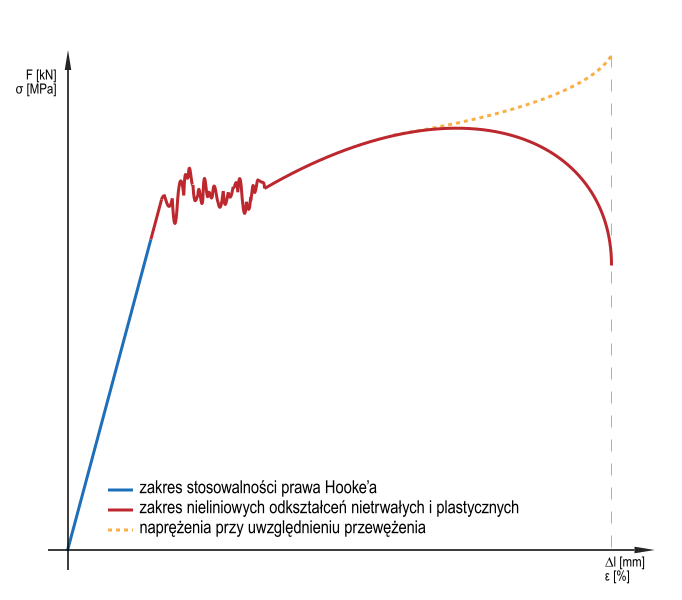
\includegraphics[scale=0.26]{tension_stress}
	\end{center}
	\vspace{-20pt}
	\caption{Zależność naprężenia od odkształcenia}
	\label{fig:tension_stress}
\end{wrapfigure}
Rysunek pokazuje typową dla metali zależność odkształcenia od naprężenia. W doświadczeniu interesuje nas przedział w którym ta
zależność jest liniowa, gdyż powyżej niej następuje trwałe odkształcenie badanego materiału i nie obowiązuje prawo Hooke'a.
Zgodnie z tym prawem zależność rozciągnięcia $\Delta l$ od siły $F$ powinna być linią prostą $\Delta l(F) = aF+b$. Porównując
to równanie prostej ze wzorem (\ref{eq:Dl}) pokazuje, że współczynnik kierunkowy jest równy $a=\frac{l}{ES}$, stąd
\begin{equation}
E=\frac{l}{aS}
\end{equation}
co po podstawieniu wzoru na pole powierzchni koła $S=\frac{\pi d^2}{4}$ daje ostateczny, roboczy wzór na moduł Younga.
\begin{equation}
\label{eq:young}
E = \frac{4l}{a*\pi d^2}
\end{equation}
Parametr $a$ tego równania będzie wyznaczany jako współczynnik prostej regresji liniowej ze zbioru wyników.

\section{Opis doświadczenia}
Do doświadczenia zostały dostarczone 2 druty, stalowy i mosiężny. Na początku zostały przeprowadzone pomiary drutów użytych w ćwiczeniu,
zmierzono ich średnicę i długość. Następnie jeden z drutów zamontowano na statywie przy pomocy nakrętek. Po wyzerowaniu śruby mikrometrycznej
następują powtarzające się czynności dokładania ciężaru na szalkę i zapisywania otrzymanych wyników. Taką samą procedurę wykonano także dla drugiego
drutu. Wyniki zapisano w tabelach.

\newpage
\section{Wyniki pomiarów}

%stalowy
\begin{table}[!htbp]
\centering
\caption{Drut stalowy}
\label{tab:drut_stalowy_wyniki}
\def\arraystretch{1.4}
\begin{tabular}{@{}rrr@{}}
\phantom{spacing} \\
długość $l$  & 1067mm & $u(l) =$~0,577mm \\	\hline
\begin{tabular}{r}średnica\\3 pomiary\end{tabular} & \multicolumn{2}{l}{0,79mm 0,79mm 0,79mm} \\	\hline
śr. średnica $\bar{d}$ & 0,79mm & $u(\bar{d}) =$~0,00577mm \\
\phantom{spacing} \\
\toprule
\multicolumn{1}{c}{\begin{tabular}[c]{@{}c@{}}Masa odważników\\ {[}kg{]}\end{tabular}} & \multicolumn{1}{c}{Ciężar {[}N{]}} & \multicolumn{1}{c}{\begin{tabular}[c]{@{}r@{}}Średnie wydłużenie\\ $\Delta$l {[}mm{]}\end{tabular}} \\ \midrule
1 & 9,81 & 0,150 \\
2 & 19,62 & 0,285 \\
3 & 29,43 & 0,400 \\
4 & 39,24 & 0,510 \\	\hline
5 & 49,05 & 0,635 \\
6 & 58,86 & 0,725 \\
7 & 68,67 & 0,855 \\	
8 & 78,48 & 0,960 \\
9 & 88,29 & 1,080 \\ \bottomrule
\end{tabular}
\end{table}
\begin{table}[!htbp]
\centering
\caption{Drut mosiężny}
\label{tab:drut_mosiezny_wyniki}
\def\arraystretch{1.3}
\begin{tabular}{@{}rrr@{}}
\phantom{spacing} \\
długość $l$  & 1067mm & $u(l) =$~0,577mm \\	\hline
\begin{tabular}{r}średnica\\3 pomiary\end{tabular} & \multicolumn{2}{l}{1,20mm 1,20mm 1,20mm} \\	\hline
śr. średnica $\bar{d}$ & 1,20mm & $u(\bar{d}) =$~0,00577mm \\
\phantom{spacing} \\
\toprule
\multicolumn{1}{c}{\begin{tabular}[c]{@{}c@{}}Masa odważników\\ {[}kg{]}\end{tabular}} & \multicolumn{1}{c}{Ciężar {[}N{]}} & \multicolumn{1}{c}{\begin{tabular}[c]{@{}r@{}}Średnie wydłużenie\\ $\Delta$l {[}mm{]}\end{tabular}} \\ \midrule
1,0 & 9,81 & 0,320 \\
2,0 & 19,62 & 0,555 \\
2,5 & 24,53 & 0,645 \\	\hline
3,0 & 29,43 & 0,730 \\
3,5 & 34,34 & 0,815 \\
4,0 & 39,24 & 0,885 \\
4,5 & 44,15 & 0,965 \\	\hline
5,0 & 49,05 & 1,040 \\
5,5 & 53,96 & 1,095 \\
6,0 & 58,86 & 1,825 \\ \bottomrule
\end{tabular}
\end{table}
\restoregeometry

\newpage
\section{Opracowanie wyników}
\begin{figure}[h]
\centerline{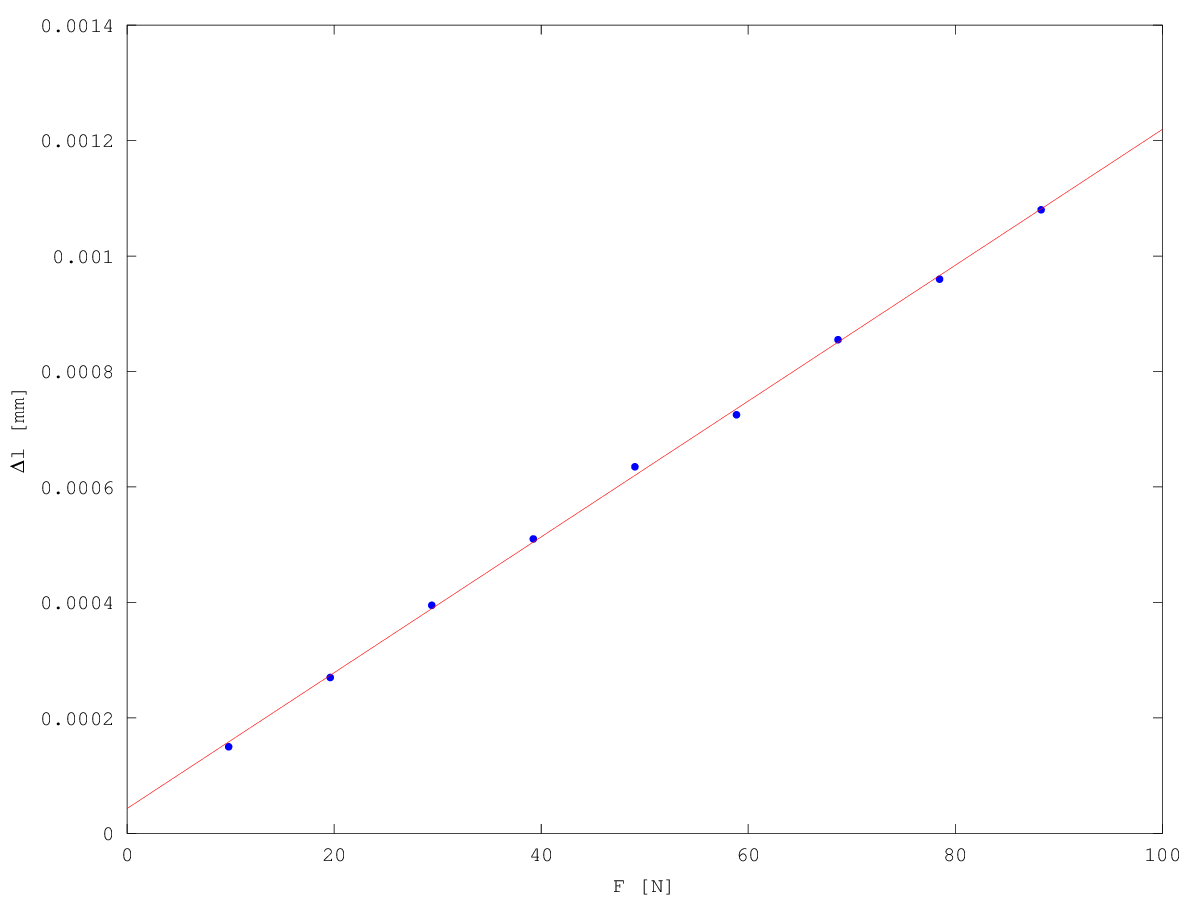
\includegraphics[scale=0.5]{image-stal}}
\caption{Wykres zależnosci odkształcenia od ciężaru dla drutu stalowego}
\label{fig:dl-stal}
\end{figure}

\begin{figure}[h]
\vspace{20pt}
\centerline{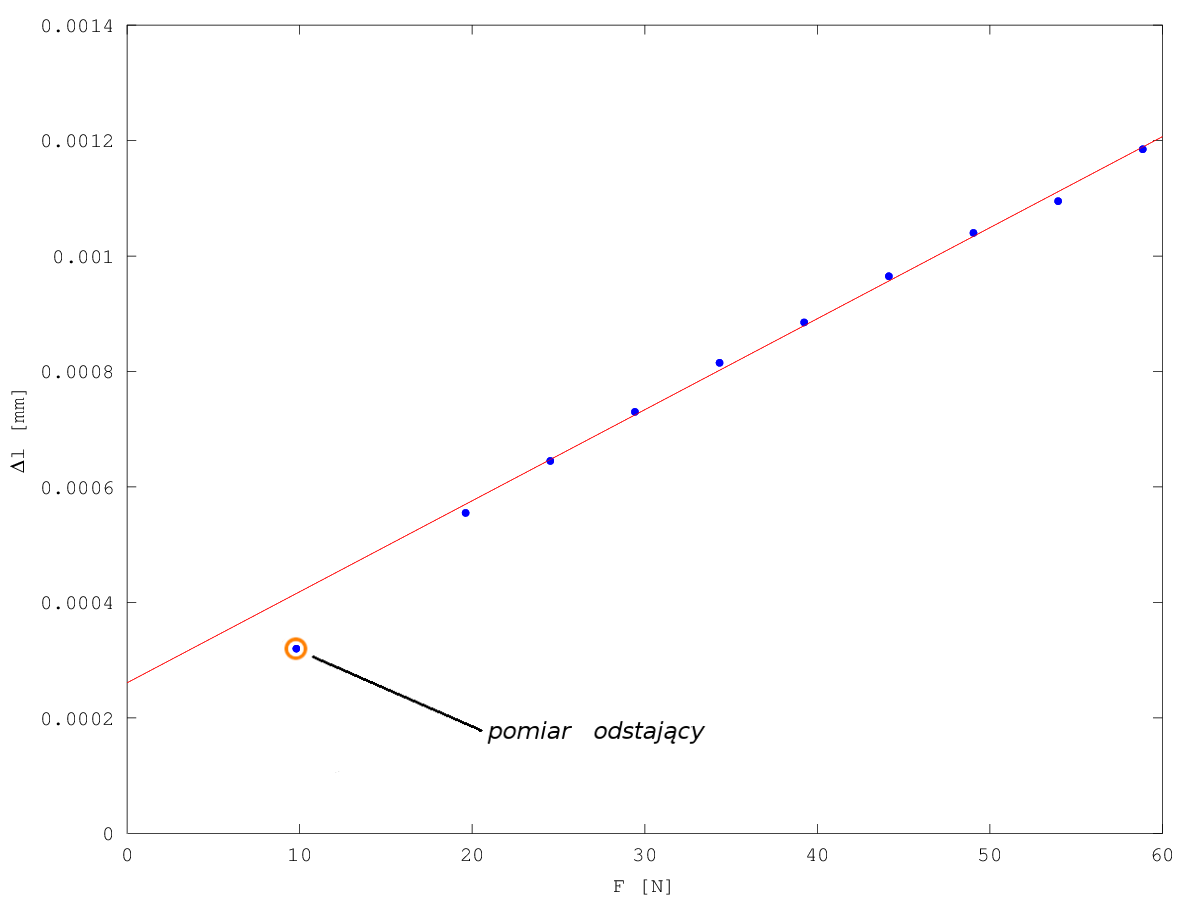
\includegraphics[scale=0.5]{image-mosiadz}}
\caption{Wykres zależnosci odkształcenia od ciężaru dla drutu mosiężnego}
\label{fig:dl-mosiadz}
\end{figure}

Wykresy na rysunkach (\ref{fig:dl-stal}) i (\ref{fig:dl-mosiadz}) przedstawiają wyniki z tabel w formie graficznej.
Niebieskimi punktami są oznaczone pomiary, a na czerwono jest zaznaczona prosta regresji liniowej. Na wykresie (\ref{fig:dl-mosiadz})
oznaczono punkt który wyraźnie odbiega od reszty, dlatego został on pominięty przy wyznaczaniu prostej regresji. Wartości te odbiegają
od oczekiwanych prawdopodobnie z powodu stanu druta mosiężnego, który był lekko powyginany.

\newpage
Wzór na moduł Younga oraz niepewność
\begin{equation*}
\begin{split}
E&=\frac{4l}{a*\pi d^2}\\
\\
u(E)&=\sqrt{\left (\frac{\partial E}{\partial a}*u(a)\right )^2+\left (\frac{\partial E}{\partial l}*u(l)\right )^2+\left (\frac{\partial E}{\partial d}*u(d)\right )^2}=\\
&=\sqrt{\left(\frac{-4*l}{a^2*\pi *d^2}*u(a)\right)^2+\left(\frac{4}{a*\pi *d^2}*u(l)\right)^2+\left(\frac{-8l}{a*\pi *d^3}*u(d)\right)^2}=\\
&= \sqrt{E^2\left (\frac{-u(a)}{a} \right )^2 + E^2\left (\frac{u(l)}{l} \right )^2 + E^2\left (\frac{-2*u(d)}{d} \right )^2}=\\
&= E\sqrt{\left (\frac{-u(a)}{a} \right )^2 + \left (\frac{u(l)}{l} \right )^2 + \left (\frac{-2*u(d)}{d} \right )^2}
\end{split}
\end{equation*}
Wartości parametru $a$ zostały wyliczone w pakiecie matematycznym.

\subsection{Drut stalowy}
\begin{equation*}
\begin{split}
a&=1.18*10^{-5}\\
E&=\frac{4*1.067}{1.18*10^{-5}*\pi*0.00079^2}\approx\\\\
&\approx 184*10^9~[Pa] = 184~[GPa]\\
\\
u(E)&=E*\sqrt{\left(\frac{-2*10^{-7}}{1.18*10^{-5}} \right )^2+\left(\frac{0.58}{1067} \right )^2+\left(\frac{-2*0.006}{0.79} \right )^2}=\\
&= E*0.02277 \approx 4*10^9 = 4~[GPa]
\end{split}
\end{equation*}

\subsection{Drut mosiężny}
\begin{equation*}
\begin{split}
a&=1.58*10^{-5}\\
E&=\frac{4*1.067}{1.58*10^{-5}*\pi*0.0012^2}\approx\\\\
&\approx 60*10^9~[Pa] = 60~[GPa]\\
\\
u(E)&=E*\sqrt{\left(\frac{-3*10^{-7}}{1.58*10^{-5}} \right )^2+\left(\frac{0.58}{1067} \right )^2+\left(\frac{-2*0.006}{1.2} \right )^2}=\\
&=E*0.02147 \approx 1*10^9 = 1~[GPa]
\end{split}
\end{equation*}

\newpage
\section{Podsumowanie}
Obliczona wartość modułu Younga dla drutu stalowego to $184 \pm 4~[GPa]$. Jest to wartość która pokrywa się z wartościami tablicowymi
wynoszącymi $\sim200~[GPa]$ i wykazującymi rozrzut około $20\%$. Jest to spowodowane tym że moduł Younga bardzo różni się dla różnych
gatunków stali w zależności od ich składu jak i sposobu obróbki.

Modułu Younga dla drutu mosiężnego jednak, wykazuje dużą rozbierzność od oczekiwanych wartości. Doświadczenia wskazują na $60 \pm 1~[GPa]$
podczas gdy tablice przewidują wartości ok. $110~[GPa]$. Jest to wartość która nie mieści się ani w niepewności zwykłej, ani rozszerzonej.
Prawdopodobnie stan drutu, jego pozaginanie jak i wiek, mogły spowodować, że otrzymane wartości są wyraźnie nienaturalne jak
dla tego materiału.

\end{document}


























